\documentclass[reprint, nobibnotes, amssymb, amsmath, amsfonts, mathtools, mathrsfs, floatfix]{revtex4-1}
\usepackage{graphicx}
\usepackage{physics}
\usepackage[english]{babel}
\usepackage{placeins}

\newcommand{\redchi}{$\tilde{\chi}^2\,$}

\newcommand{\moss}{M\"{o}ssbauer }

\begin{document}

  \title{\moss Spectroscopy of Fe-57}

  \author{Aman LaChapelle}
  \affiliation{The University of Chicago}

  \begin{abstract}
    We use \moss spectroscopy to determine several properties of excited Fe-57.  Using Stainless Steel, we measure the linewidth of the excited state of Fe-57 to be $(2.0\pm0.1)e-08\,\, eV$, corresponding to a lifetime of $66 \pm 3\,\, ns$.  We measure an isomer shift of $\delta = (-1.21\pm0.03)e-08\,\, eV$, with $\delta$ the distance from 14.4 keV.  We also use a magnetic Fe-57 sample to measure the Zeeman splitting of nuclear energy levels $\Delta E_1 = -(1.0\pm0.2)e-7\,\, eV$ and $\Delta E_0 = (1.8\pm0.4)e-7\,\, eV$, a nuclear magnetic moment of the excited state of $\mu_1 = -(0.15\pm0.06)\mu_N$ and the magnetic field at the nucleus of $32\pm12\,\, T$.  Finally, we make use of an electric quadrupole sample in order to determine $\tilde{Q}\frac{\partial E}{\partial z} = (3.2\pm0.3)e-7 \,\, V$ at the Fe-57 atom, and find $\frac{\partial E}{\partial z} = (1.5\pm0.1)e-6\,\, V/barn$ at the atom.
  \end{abstract}

  \maketitle
  \tableofcontents

  \section{Introduction and Theory}
    We seek to perform a number of measurements using the technique of \moss spectroscopy.  The principle is that we are able to use doppler shift to measure energies at remarkably tiny scales.  We will achieve incredibly high precision in our measurements by using a fixed source that we move with a known velocity in order to make use of the doppler shift phenomenon to alter the energy of the source by a tiny amount.  We need this high resolution because the phenomena we are measuring take place and induce shifts of the order of $10^{-7}$ eV, and this causes difficulty for many experiments.  Other types of experiments are also able to examine phenomena with resolution like the \moss technique, but are by far more complicated, and furthermore measure different phenomena in general.  Many AMO experiments make use of lasers and sub-MHz resolution to examine similar features of nuclei, but their setups are far more complicated and experiments are much more time-intensive and expensive.  Therefore, in order to measure nuclear phenomena in metallic crystals, we make use of this \moss technique.

    In general when an excited atom emits a photon, the atom will recoil.  However, if these atoms are confined in a crystal lattice, the entire lattice may recoil.  If, however, absorption is to occur, then both processes must be recoilless, and the photon shift due to nuclear recoil will be much smaller because of the massive number of atoms confined in the lattice.  In fact, the absorption and emission spectra will overlap in these cases.  We examine perturbational effects that cause the transition energy to shift or split, specifically Isomer shift, the Zeeman effect, and Quadrupole splitting.

    We need a few more things in order to proceed.  Since we are observing a dip in the transmission spectrum which is a convolution of 2 lorentzian functions (the absorption and emission spectra), the actual linewidth of the state is about half the observed/fitted linewidth,
    \begin{equation}
      \Gamma_{obs} \approx 2 \Gamma. ~\label{linewidths}
    \end{equation}

    Finally, in order to actually use $\Gamma$ to calculate the lifetime of a state, we use the energy-time uncertainty relation in the following way,
    \begin{equation}
      \Delta E \Delta t = \frac{\Gamma}{2}\tau = \frac{\hbar}{2}. ~\label{lifetimes}
    \end{equation}

    \subsection{Isomer Shift}
      This effect emerges from the embedding of a nucleus in a heterogeneous chemical environment.  In our case we work with Stainless Steel, alloy 302, whose chemical composition is outlined in Table~\ref{tab:SS_chemical_makeup}.  Approximately 70\% of the alloy is Iron, and of that only a tiny percentage (approx. 1\%) is Fe-57.  This is an ideal environement to see the isomer shift because it is enough Fe-57 that we will be able to see a peak develop, but not so much that we have more excited iron than other chemicals and so our isomer shift will be strong and present.  We can determine the energy of the shifted transition with the following:
      \begin{equation}
        E_{iso} = \delta + E_0 \label{isomer_shift}
      \end{equation}
      with $E_0$ being the energy before the shift, $\delta$ being the isomer shift, and $E_{iso}$ being the energy after the shift.  We know that the transition we are looking for has a certain energy, and by fitting the transition dip that we see from our \moss spectrum, we will be able to determine $E_{iso}$.  In our plots, as we will see, we have centered around $E_0$, so we measure delta directly.

      It is important to note that the following effects stack onto the isomer shift, which is the mechanism by which we shift the first peak/transition.  These other effects simply further split this transition.

      \subsection{Zeeman Splitting}
        When we place an atom in a magnetic field, the magnetic moments of the electrons and the nucleus begin to have a dependence on chirality - that is, it will have more energy cost to have your magnetic moment antiparallel to the external $\vec{H}$ field.  We thus introduce a perturbation to the Hamiltonian:
        \begin{equation}
          H_{Zeeman} = -\mu \cdot \vec{H}.
        \end{equation}
        We can define the magnetic moment in terms of the gyromagnetic ratio and the angular momentum of the nucleus, and then take the first order energy perturbation to find the energy shift:
        \begin{equation}
          \Delta E_{Zeeman} = \frac{\mu}{I}|\vec{H}|m_{I}
        \end{equation}
        where $I$ is the eigenvalue of total angular momentum, and $m_I$ is the eigenvalue of the z-component.

        Since there are two energy levels, and each will split, we will see a total of 6 transitions (this is clear if we look at Figure~\ref{zeeman_shifts}).  We can calculate the splitting between adjacent states - states of different $m_I$ - to be the following:
        \begin{gather}
          \Delta E_1 = \mu_1|H|/I_1 \label{E1_zeeman_shift} \\
          \Delta E_0 = \mu_0|H|/I_0 \label{E2_zeeman_shift}
        \end{gather}
        We can measure $\Delta E_{1}$ by taking two adjacent measurements (for example, the first and second) and subtracting them.  We can do the same for $\Delta E_{0}$, but we can only do this for the 3rd and 4th measurements, all the other pairs measure $\Delta E_1$ only.

      \subsection{Quadrupole Splitting}
        If we place a nucleus in a region with an electric field gradient, we will see the charge distribution change its shape depending on the charge interactions.  We classify the Quadrupole moment $Q$ as being positive if the long axis of the ellipsoid is along the $\hat{z}$ field, negative if it is perpendicular and zero if the distribution is spherically symmetric.  The ground state of Fe-57 is spherically symmetric and so has $Q = 0$, but the first excited state is not and will therefore split in a region with a field gradient.  The quadrupole moment $Q$ defined in terms of the intrinsic quadrupole moment $\tilde{Q}$, and the energy shift are defined as:
        \begin{gather}
          Q = \frac{3 m_I^2 - I(I+1)}{I(2I-1)}\tilde{Q} \label{quadrupole_moment} \\
          \Delta E = \frac{1}{4}eQ\frac{\partial E}{\partial z} = \frac{e\left(3 m_I^2 - I(I+1)\right)}{4I(2I-1)}\tilde{Q}\frac{\partial E}{\partial z} \label{quadrupole_shift}
        \end{gather}
        We do not measure this exactly, however.  We measure the transition from the $I = 1/2,\,\, m_I = \pm1/2$ state into the $I = 3/2,\,\, m_I = \pm1/2, \pm3/2$ states.  Adopt Dirac notation, with $\ket{I, m_I}$.  We can thus measure this $\Delta E$ by taking $\ket{1/2,\,\pm1/2} \rightarrow \ket{3/2,\,\pm3/2}$ and subtracting $\ket{1/2,\,\pm1/2} \rightarrow \ket{1/2,\,\pm1/2}$.  This is made much clearer by taking a short look at Figure~\ref{quadrupole_shifts}.

  \section{Methods and Calibration}
    \subsection{Methods}
      Throughout this section, we will refer to items that are labeled in Figure~\ref{apparatus}.  The reader should therefore keep Figure~\ref{apparatus} close at hand, it will simplify this section greatly.

      We begin with the Co-57 source, which decays to an excited Fe-57 nucleus by electron capture.  The energy splitting between the states that we care about is at 14.4 keV.  If we look at the decay scheme, Figure~\ref{co_57}, we will see that the only photons that are emitted far from other photons (such as the ones emitted by Pd and Pb) are the ones emitted at 14.4 keV.  Thus if we exclude the x-ray spectrum with a filter, the only photons emitted are at 14.4 keV.

      The Co-57 source does, however, only emit at a certain energy.  We need to be able to scan the energy, so we attach this to a linear motor, which allows us to use the doppler shift of photons emmited from a moving source to scan in energy.  This movement is very slow - around $\pm1$ cm/sec, which is less than $10^{-10} c$, and so we can resolve extremely tiny features on the spectrum with relatively low overhead.

      In order to actually be able to calibrate anything, however (which we will explain in more detail in the next section), we must realize that we have to measure this movement and its velocity.  We do this by attaching and aligning a michelson interferometer to the other end of the sample arm (with the linear drive), and we measure the velocity by counting fringes that pass by on the photocell.

      We count the fringes using a Multi-Channel Scaler (MCS) which divides units of time into discrete chunks that can be managed by a channel-based collection software package.  We set the dwell time to 300 $\mu s$ and the MCS correlates veolcity to channel as divided by our set dwell time.

      We've established the apparatus that allows us to sweep energy and tell us how we are sweeping the energy.  We have not, however, established how we are actually taking the data, capturing the photons after they interact with the target.  For this we use a proportional counter - a gas-filled chamber.  As photons that pass through the target interact with the gas, we see electrons ejected from atoms, which then ionize other atoms, which then forms a cascade on a central wire, which is what we actually measure.  An operating voltage is chosen such that the total number of electrons (and thus the cascade) is proportional to the energy of the photon.  From here the voltages are fed into the pulse height analyzer (PHA), which bins the data according to discrete voltage steps into channels.

    \subsection{Calibration}
      Since the PHA takes data as counts vs channel, we need to be able to take the channels and convert them to energy.  The way we do this is by using the velocity spectrum shown in Figure~\ref{velocity_plot}.  This is a plot of the velocity of the sample in the sense that each bin contains the number of times that the sample was moving at that particular velocity.  This is determined, as we saw earlier, by fringe counting.  We can thus convert from channel to velocity like so:
      \begin{gather}
        counts(channel) = A(channel - C) \\
        v(channel) = \frac{counts(channel)\,\lambda}{2 n \Delta t} \label{calibration}
      \end{gather}
      where $\lambda$ is the known wavelength of the laser (632.8 nm), $\Delta t$ is the dwell time, 300 $\mu s$, n is the number of passes that were made by the sample (the number of times that the sample moved back and forth, in this case 116) and A and C we fit in Figure~\ref{velocity_plot} to determine with high precision.  The number of fringes is the $counts(channel)/n$, which is what we count in the PHA (which we are converting from now).  From this we can determine the energy shift off of 14.4 keV by taking
      \begin{equation}
        \delta = \frac{v(channel)}{c}E = \frac{v(channel)}{2.9979e+08} 14.4e+03\,\,eV \label{vel_to_energy}
      \end{equation}
      which allows us to find and fit the transitions to incredible precision.

      We might think that the calibration would be unstable and it is possible that this calibration would change if we were taking data over two days, but we were able to finish taking our data on the first day, and even though we took 3 velocity calibration plots, they were all nearly (to better than 0.01\%) identical in fit parameters and therefore in calibration - so we can assume that our calibration did not drift much if at all.  This all leads us to the conclusion that the calibration was \textbf{not} a major source of uncertainty in this experiment.

  \section{Discussion and Analysis}
    \subsection{Stainless Steel/Isomer Shift}
      If we take a look at Figure~\ref{ss_fit} and its associated table (Table~\ref{tab:ss_fit_stats}), we will notice a few things.  Perhaps the first thing to notice is that the \redchi value is 2.09.  This seems large for such a good fit.  This is well-explained, however.  Off to the left side of the plot there is a residual feature, the origin of which is likely due to some jitter in the spectrum or possibly where the carriage turns around, causing lower counts for some reason.  If we exclude this feature and recalculate the \redchi value, we return 1.13, which is much more in line with what we would expect.

      From the other two values, $\delta$ and $\Gamma$, we can extract the isomer shift and the linewidth of this excited state.  Since we have $\delta$ already, we use equation~\ref{isomer_shift} to calculate $E_{iso}$.  This calculation is extremely straightforward, and we return a value of $14.3999999999879 \pm 0.00000000003$ keV.  This is obviously a tiny difference and a ridiculous number to carry around, so going forward we will report all energies in terms of the difference from 14.4 keV, that is, just report $\delta$.

      From $\Gamma = (2.0 \pm 0.1)e-08 \,\, eV$, we can use eq.s~\ref{linewidths} and~\ref{lifetimes} to calculate $\tau$, the mean lifetime of the state.  Plugging all the numbers in, we find that $\tau = 66\pm3\,\, ns$.  This is not within uncertainties of the expected value of 98 ns.  Because many of our other values are so close to the expected values, this may be because of the assumption that we make in equation~\ref{linewidths}, but we are not truly sure.

    \subsection{Zeeman Splitting}
      Changing gears to the enriched Fe-57 spectrum (Figure~\ref{fe_fit} ), where we will identify the Zeeman peaks and find the energy splittings~\ref{E1_zeeman_shift} and~\ref{E2_zeeman_shift}.  Looking at Figure~\ref{zeeman_shifts}, we can see that any two adjacent peaks that are not the 3rd and 4th (counting from the left) will give us $\Delta E_1$ and the difference between peaks (say) 2 and 4 will give us $\Delta E_0$.  If we reference Table~\ref{tab:fe_57_fit} and take two adjacent peaks that are not peaks 3 and 4, say 1 and 2, we will see that $\delta_1 = -2.53e-07 \pm 1.7e-08 \,\, eV$ and $\delta_2 = -1.51e-07 \pm 1.7e-08 \,\, eV$.  Then
      \begin{equation}
        \delta_2 - \delta_1 = \Delta E_1 = -(1.0\pm0.2)e-07 \,\, eV.
      \end{equation}
      We add fractional uncertainties directly because although in an ideal world the uncertainties would be independent, the reality is that for this particular fit (which we have performed on many datasets many times), tends to depend strongly on other peak positions (the peaks depend strongly on each other).  So we take the uncertainties to be co-dependent and add fractional uncertainties directly.  Recall that uncertainties are found by choosing random points within the distribution about each individual point and iterating the fit 300 times to minimize statistical error and reduce uncertainties to just fit uncertainties.

      In order to find $\Delta E_0$, we take peaks 2 and 4, and subtract.
      \begin{equation}
        \Delta E_0 = |\delta_4 - \delta_2| = (1.8\pm0.4)e-07 \,\, eV
      \end{equation}
      where here we take the absolute value (even though it is not strictly necessary) after the subtraction because one peak is to the right of 14.4 keV and one is to the left (one has been shifted up and the other down), so we want the total distance between the two.  Again, we take uncertainties to be related for the same reasons as before, and so we add fractional uncertainties directly.

      Now that we have $\Delta E_0$ and $\Delta E_1$, we can calculate $\mu_0$ and $\mu_1$ as follows, by beginning with the ratio - dividing eq.~\ref{E1_zeeman_shift} by eq.~\ref{E2_zeeman_shift}.
      \begin{gather}
        \frac{\Delta E_0}{\Delta E_1} = \frac{\mu_0 \abs{\vec{H}}}{I_0} \frac{I_1}{\mu_1 \abs{\vec{H}}} \\
        \frac{\Delta E_0}{\Delta E_1} = \frac{\mu_0 I_1}{\mu_1 I_0} \\
        \frac{\Delta E_0}{\Delta E_1} = -1.8 = \frac{\mu_0 (3/2)}{\mu_1 (1/2)} \\
        \frac{\mu_0}{\mu_1} = -0.6 \pm 0.2
      \end{gather}
      The uncertainty is quite large - this is because we added the fractional uncertainties in the peak positions directly, and then since the underlying source of uncertainty is the same, we realize that we have to add fractional uncertainties directly yet again.  This yields a large uncertainty that we can't deflate any further.  We are so close to the literature values that it seems as though we could decrease these uncertainties by adding in quadrature at least, but lacking in convincing evidence to do so we leave them as they are.

      Using the value for $\mu_0$ given in~\cite{lab_manual}, we can then calculate $\mu_1$, and we find that
      \begin{equation}
        \mu_1 = -(0.15\pm0.06)\mu_N
      \end{equation}
      The accepted literature value is $\mu_1 = -0.1546\,\mu_N$~\cite{mu_1}, and we are definitely within uncertainty of this value.  From this, we can calculate the magnetic field at the sample, using equation~\ref{E2_zeeman_shift}, and return
      \begin{equation}
        |\vec{H}| = \frac{\Delta E_1 I_1}{\mu_1} = \frac{-1.0e-7 \cdot 3/2}{-0.15 \mu_N} = \frac{1e-6 eV}{\mu_N} = (32\pm12) T.
      \end{equation}

    \subsection{Quadrupole Splitting}
      Finally, we deal with one more perturbation, the Quadrupole moment shift caused by an electric field gradient.  We see this effect in Figure~\ref{quadrupole_fit}, and we can find fit values in Table~\ref{tab:quad_fit}.  Now, looking at Figure~\ref{quadrupole_shifts}, we notice that $\Delta E_{quad}$ can be found by subtracting the location of the second peak (again, count from the left) from the location of the first peak.  If we do this, we find
      \begin{equation}
        \Delta E_{quad} = \delta_2 - \delta_1 = (8.1 \pm 0.8)e-8 \,\, eV
      \end{equation}
      From this, we can make use of equation~\ref{quadrupole_shift} and plug in $I = 3/2$ and $m_I = 3/2$ - if we use $m_I = 1/2$ we get the negative of our answer so we choose the positive value,
      \begin{gather}
        \frac{\Delta E_{quad} \cdot 4I(2I-1)}{e\left(3 m_I^2 - I(I+1)\right)} = \tilde{Q}\frac{\partial E}{\partial z} \\
        \tilde{Q}\frac{\partial E}{\partial z} = (3.2\pm0.3)e-7 \,\, V
      \end{gather}
      So given $\tilde{Q} \approx 0.1-1.0 \,\, barn \approx (0.1-1.0)e-28 \,\, m^{2}$, this means that our electric field gradient is, in SI units (choose $\tilde{Q} = 0.21\,\, barn$\cite{field_gradient}),
      \begin{equation}
        \frac{\partial E}{\partial z} = (1.5\pm0.1)e+22 \,\, V/m^2
      \end{equation}
      or in more sensible units
      \begin{equation}
        \frac{\partial E}{\partial z} = (1.5\pm0.1)e-6\,\, V/barn.
      \end{equation}
      where we have taken uncertainties in the value of $\tilde{Q}$ to be much smaller than the uncertainties in our own experiment (and thus negligible), which were taken to be 9\%.  As we can see, if we consider the field gradient in SI units the value is huge.  This is of course due to the size of the molecule, which is on the order of barns not on the order of square meters.  This is clear when we look at the field gradient in more sensible units and see that it is quite small over the range that we are considering, and makes sense that it would split the line by the amount that it does.  The only thing that we were able to find on the field gradient says that it is roughly $0.585e+18 V/cm^2 \approx 0.585e+22 V/m^2$~\cite{na_nitroprusside}.  We are unsure of how significant this is, mostly because we don't understand much of the methodology or the paper itself.  However, this does seem to indicate that we are at least on the right order of magnitude.

  \section{Conclusion, Tables and Figures}
    We have, where appropriate, established how close our measured values are to the accepted literature values, we have established how we propagate uncertainties, and we have understood the precision afforded us by the \moss technique.

    Our fits were overall excellent given their complexity in functional form and in the variable space that the minimizer had to conquer.  We believe that our \redchi values were driven up by the few points to the left side of each figure where we can see there is some defect of the counting apparatus.  In every case when we remove that part of the spectrum our \redchi values move closer to 1, but we cannot be certain that these points are indeed a defect and not another feature, and as such we cannot rule them out.

    In the future perhaps calibrations can be taken only at the beginning and end of the day, because as we saw, the calibration didn't drift much if at all.

    This work was undertaken with Will Harrison and Kris Pittard.  Our thanks to the staff of the Advanced Undergraduate Physics Laboratories for their patience and helpful hands, especially Brian Mohs for reading this almost painfully long report not once but twice.  For the final P211 experiment of 2016, a special thanks to Dave McCowan for his many hours of hard work (especially the wiki), good humour and willingness to answer questions all year long.  Shoutout to Van Bistrow for being good-natured about most everything and patient in the face of adversity.

    \subsection{Tables}
      \FloatBarrier
      \begin{table}[h]
        \centering
        \begin{tabular}{|c|c|}
          \hline
          Element & Content (\%) \\ \hline
          Cr & 17-19 \\ \hline
          Ni & 8-10 \\ \hline
          Mn & 2 \\ \hline
          Si & 1.00 \\ \hline
          C & 0.15 \\ \hline
          S & 0.03 \\ \hline
          P & 0.045 \\ \hline
        \end{tabular}
        \caption{The remainder is Fe, mostly Fe-56.~\cite{stainless_chemical_makeup}~\label{tab:SS_chemical_makeup}}
      \end{table}

      \begin{table}[h]
        \centering
        \begin{tabular}{|c|c|c|}
          \hline
          Quantity & Value & Uncertainty \\ \hline \hline
          $I_0$ ($eV/s/m^2$) & 7.13e+02 & 2.5e+01 \\ \hline \hline
          $\Gamma$ ($eV$) & 2.0e-08 & 1e-09 \\ \hline \hline
          $\delta$ ($eV$) & -1.21e-08 & 3e-10 \\ \hline \hline
          $C$ & 1574 & 3 \\ \hline
        \end{tabular}
        \caption{Fit values for our Stainless Steel spectrum.  The covariance matrix for this fit was well-defined, so the uncertainties on this fit simply come from the diagonals of the covariance matrix.~\label{tab:ss_fit_stats}}
      \end{table}

      \begin{table}[h]
        \centering
        \begin{tabular}{|c|c|c|}
          \hline
           Quantity (indexed by peak) & Value & Uncertainty \\ \hline \hline
           $I_{0, 1}$ ($eV/m^2/s$) & 4.3e+02 & 8e+01 \\ \hline
           $I_{0, 2}$ ($eV/m^2/s$) & 3.9e+02 & 9e+01 \\ \hline
           $I_{0, 3}$ ($eV/m^2/s$) & 2e+02 & 10e+01 \\ \hline
           $I_{0, 4}$ ($eV/m^2/s$) & 2.5e+02 & 7e+01 \\ \hline
           $I_{0, 5}$ ($eV/m^2/s$) & 3.7e+02 & 8e+01 \\ \hline
           $I_{0, 6}$ ($eV/m^2/s$) & 3.8e+02 & 9e+01 \\ \hline \hline
           $\Gamma_1$ ($eV$) & 1.6e-08 & 1e-09 \\ \hline
           $\Gamma_2$ ($eV$) & 1.4e-08 & 2e-09 \\ \hline
           $\Gamma_3$ ($eV$) & 1.3e-08 & 3e-09 \\ \hline
           $\Gamma_4$ ($eV$) & 1.6e-08 & 2e-09 \\ \hline
           $\Gamma_5$ ($eV$) & 1.6e-08 & 3e-09 \\ \hline
           $\Gamma_6$ ($eV$) & 2.0e-08 & 3e-09 \\ \hline \hline
           $\delta_{1}$ ($eV$) & -2.53e-07 & 1.7e-08 \\ \hline
           $\delta_{2}$ ($eV$) & -1.51e-07 & 1.7e-08 \\ \hline
           $\delta_{3}$ ($eV$) & -4.57e-08 & 1.7e-08 \\ \hline
           $\delta_{4}$ ($eV$) & 3.27e-08 & 1.7e-08 \\ \hline
           $\delta_{5}$ ($eV$) & 1.41e-07 & 1.7e-08 \\ \hline
           $\delta_{6}$ ($eV$) & 2.52e-07 & 1.7e-08 \\ \hline \hline
           $C_1$ (counts) & 2.34e+03 & 2e+01 \\ \hline
           $C_2$ (counts) & 2.30e+03 & 2e+01 \\ \hline
           $C_3$ (counts) & 2.300e+03 & 1.4e+01 \\ \hline
           $C_4$ (counts) & 2.30e+03 & 2e+01 \\ \hline
           $C_5$ (counts) & 2.300e+03 & 1.5e+01 \\ \hline
           $C_6$ (counts) & 2.300e+03 & 1.2e+01 \\ \hline
        \end{tabular}
        \caption{Fit values for Fe-57.  $\delta$ signifies distance from the center, which is set to 14.4 keV.  The covariance matrix was not well-defined so uncertainties were determined by running the fit on randomized points chosen from a normal distribution around each points best-guess value, iterating 300 times, and taking the standard deviation of those values.  The values of C from 2 to 6 are the same because of the way that the fit was performed - there was a bias so that those values would end up the same to reduce the computational intensity of the fitting function.  The uncertainties were different, so we decided to show them all anyway.~\label{tab:fe_57_fit}}
      \end{table}

      \begin{table}[h]
        \begin{tabular}{|c|c|c|}
          \hline
          Quantity (indexed by peak) & Value & Uncertainty \\ \hline \hline
          $I_{0, 1}$ ($eV/m^2/s$) & 3.26e+02 & 6e+00 \\ \hline
          $I_{0, 2}$ ($eV/m^2/s$)& 3.9e+02 & 3e+01 \\ \hline \hline
          $\Gamma_1$ ($eV$) & 1.4e-08 & 2e-09 \\ \hline
          $\Gamma_2$ ($eV$) & 9.85e-09 & 6e-10 \\ \hline \hline
          $\delta_{1}$ ($eV$) & -6.0e-08 & 4e-09 \\ \hline
          $\delta_{2}$ ($eV$) & 2.1e-08 & 4e-09 \\ \hline \hline
          $C_1$ (counts) & 3.0e+03 & 3e+02 \\ \hline
          $C_2$ (counts) & 2.3e+03 & 3e+02 \\ \hline
        \end{tabular}
        \caption{Fit values for the Quadrupole sample.  $\delta$ signifies distance from the center, which is set to 14.4 keV.  Again, the covariance matrix was not well-defined so we used the method of running the fit on randomly chosen data points within the normal distribution centered at each best-guess point.  The standard deviation converged in just under 100 runs for this case, so we used 100 iterations.~\label{tab:quad_fit}}
      \end{table}

      \FloatBarrier

    \subsection{Figures}
    \begin{widetext}
      \FloatBarrier

      \begin{figure}[h]
        \centering
        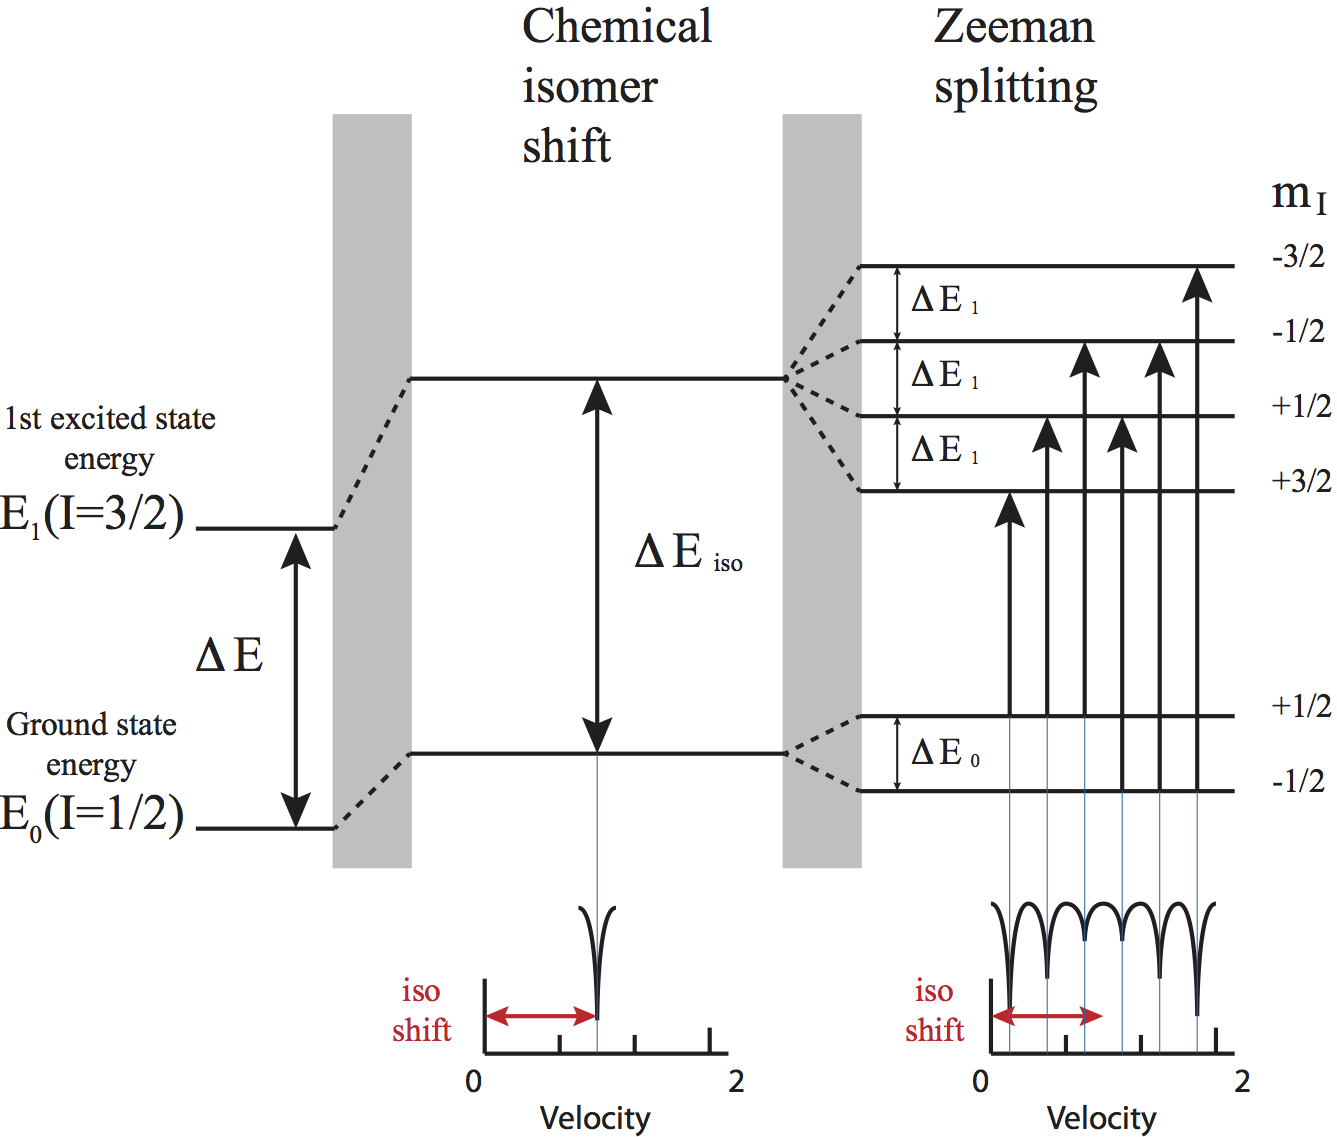
\includegraphics[width=\linewidth]{Mossb_energy_shifts_zeeman.png}
        \caption{A diagram to help visualize the Zeeman energy perturbations - this cleanly describes the appearance of 6 peaks/transitions.~\cite{lab_manual}~\label{zeeman_shifts}}
      \end{figure}

      \begin{figure}[h]
        \centering
        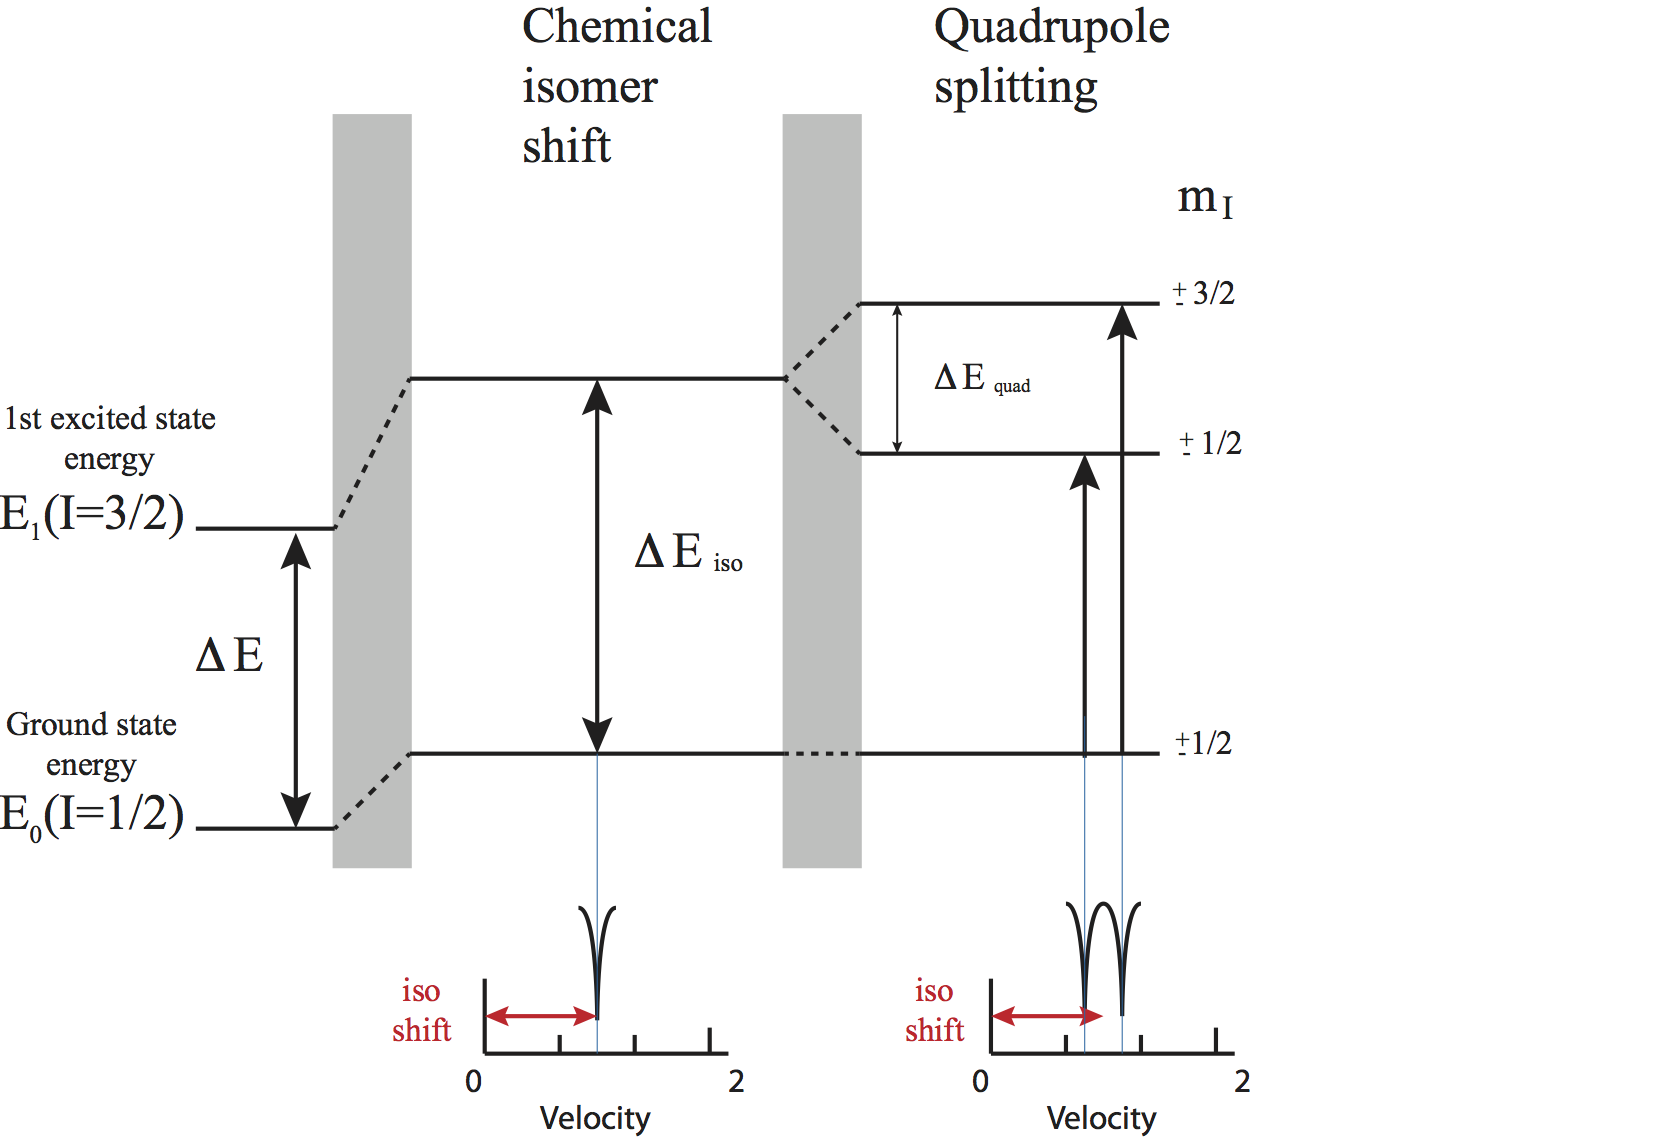
\includegraphics[width=\linewidth]{Mossb_quad_shifts.png}
        \caption{Another visualization of the energy level splittings, this illustrates the way that we will measure the splitting itself.~\cite{lab_manual}~\label{quadrupole_shifts}}
      \end{figure}

      \begin{figure}[h]
        \centering
        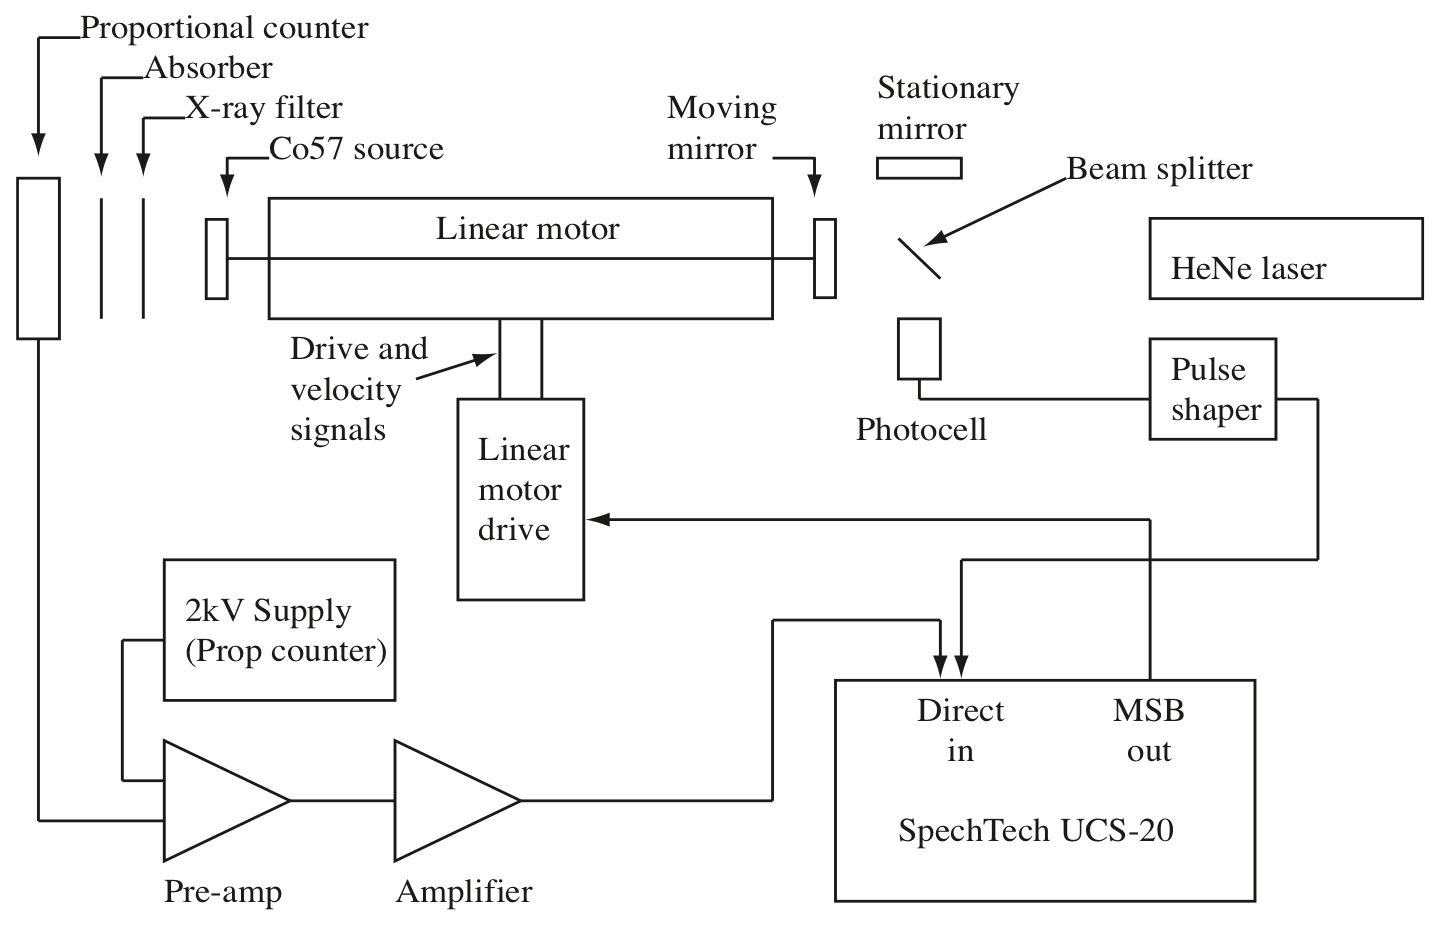
\includegraphics[width=\linewidth]{apparatus.png}
        \caption{A block diagram of the \moss apparatus.  We likely would not have been able to render anything better by hand, but this gives the general idea as well as a rudimentary signal path diagram.~\cite{lab_manual}~\label{apparatus}}
      \end{figure}

      \begin{figure}[h]
        \centering
        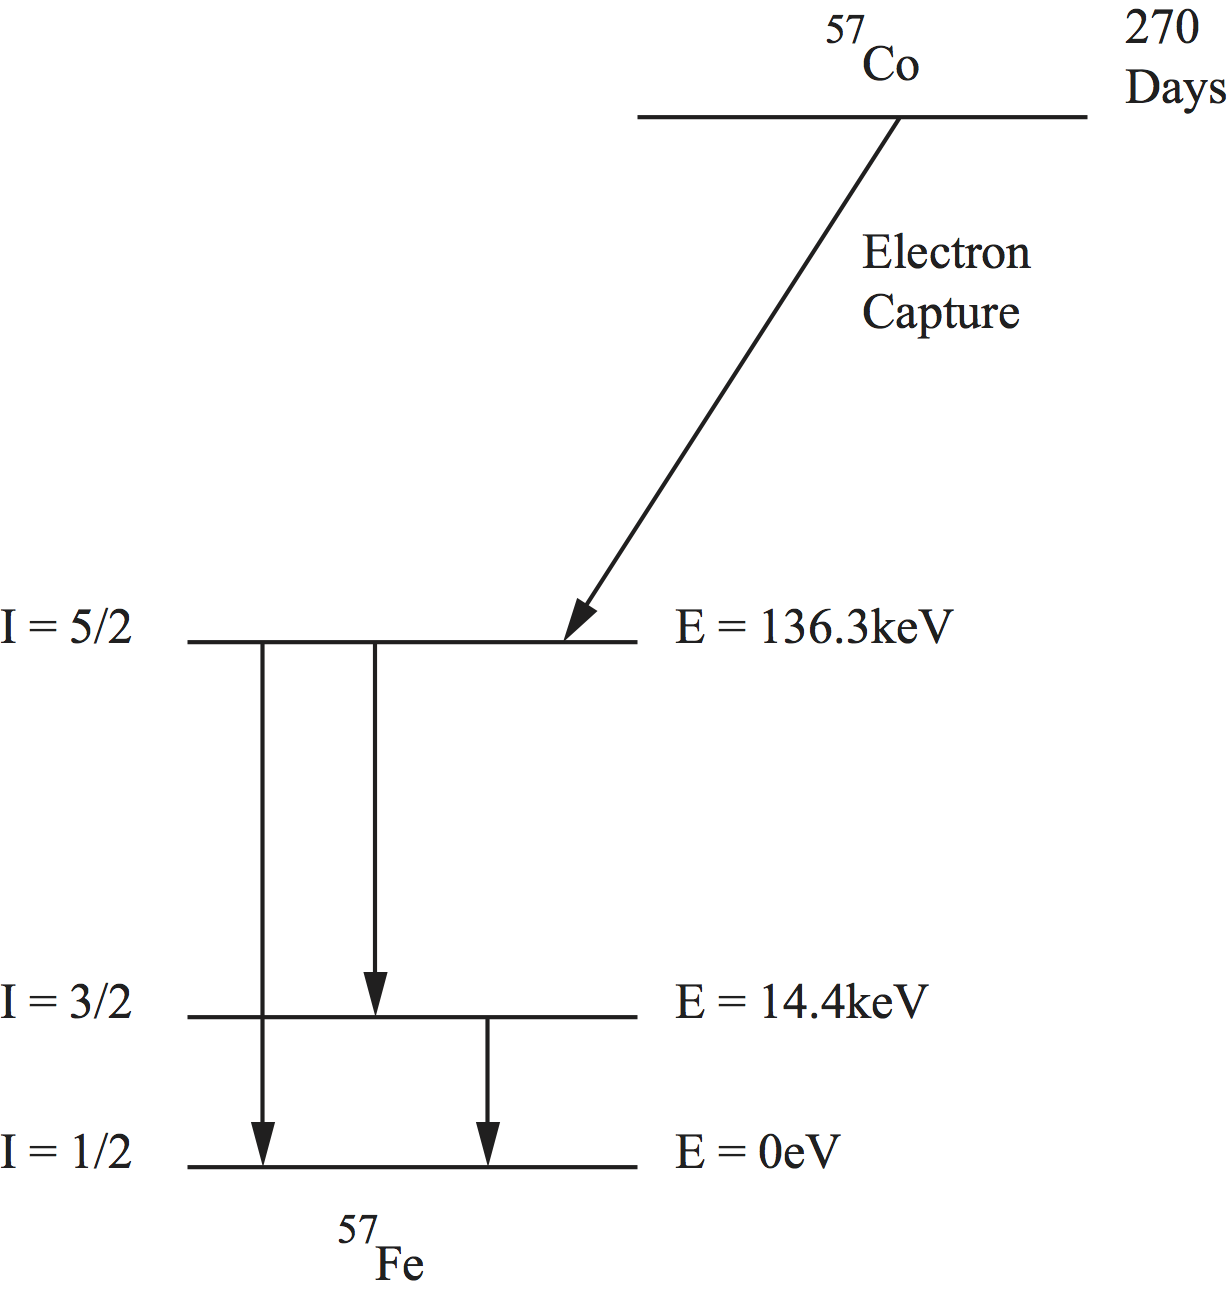
\includegraphics[width=\linewidth]{Co_57_decay.png}
        \caption{The decay scheme for Co-57 - illustrative of our efforts to examine the changes in energy levels at $I = 1/2$ and $I = 3/2$~\cite{lab_manual}~\label{co_57}}
      \end{figure}

      \begin{figure}[h]
        \centering
        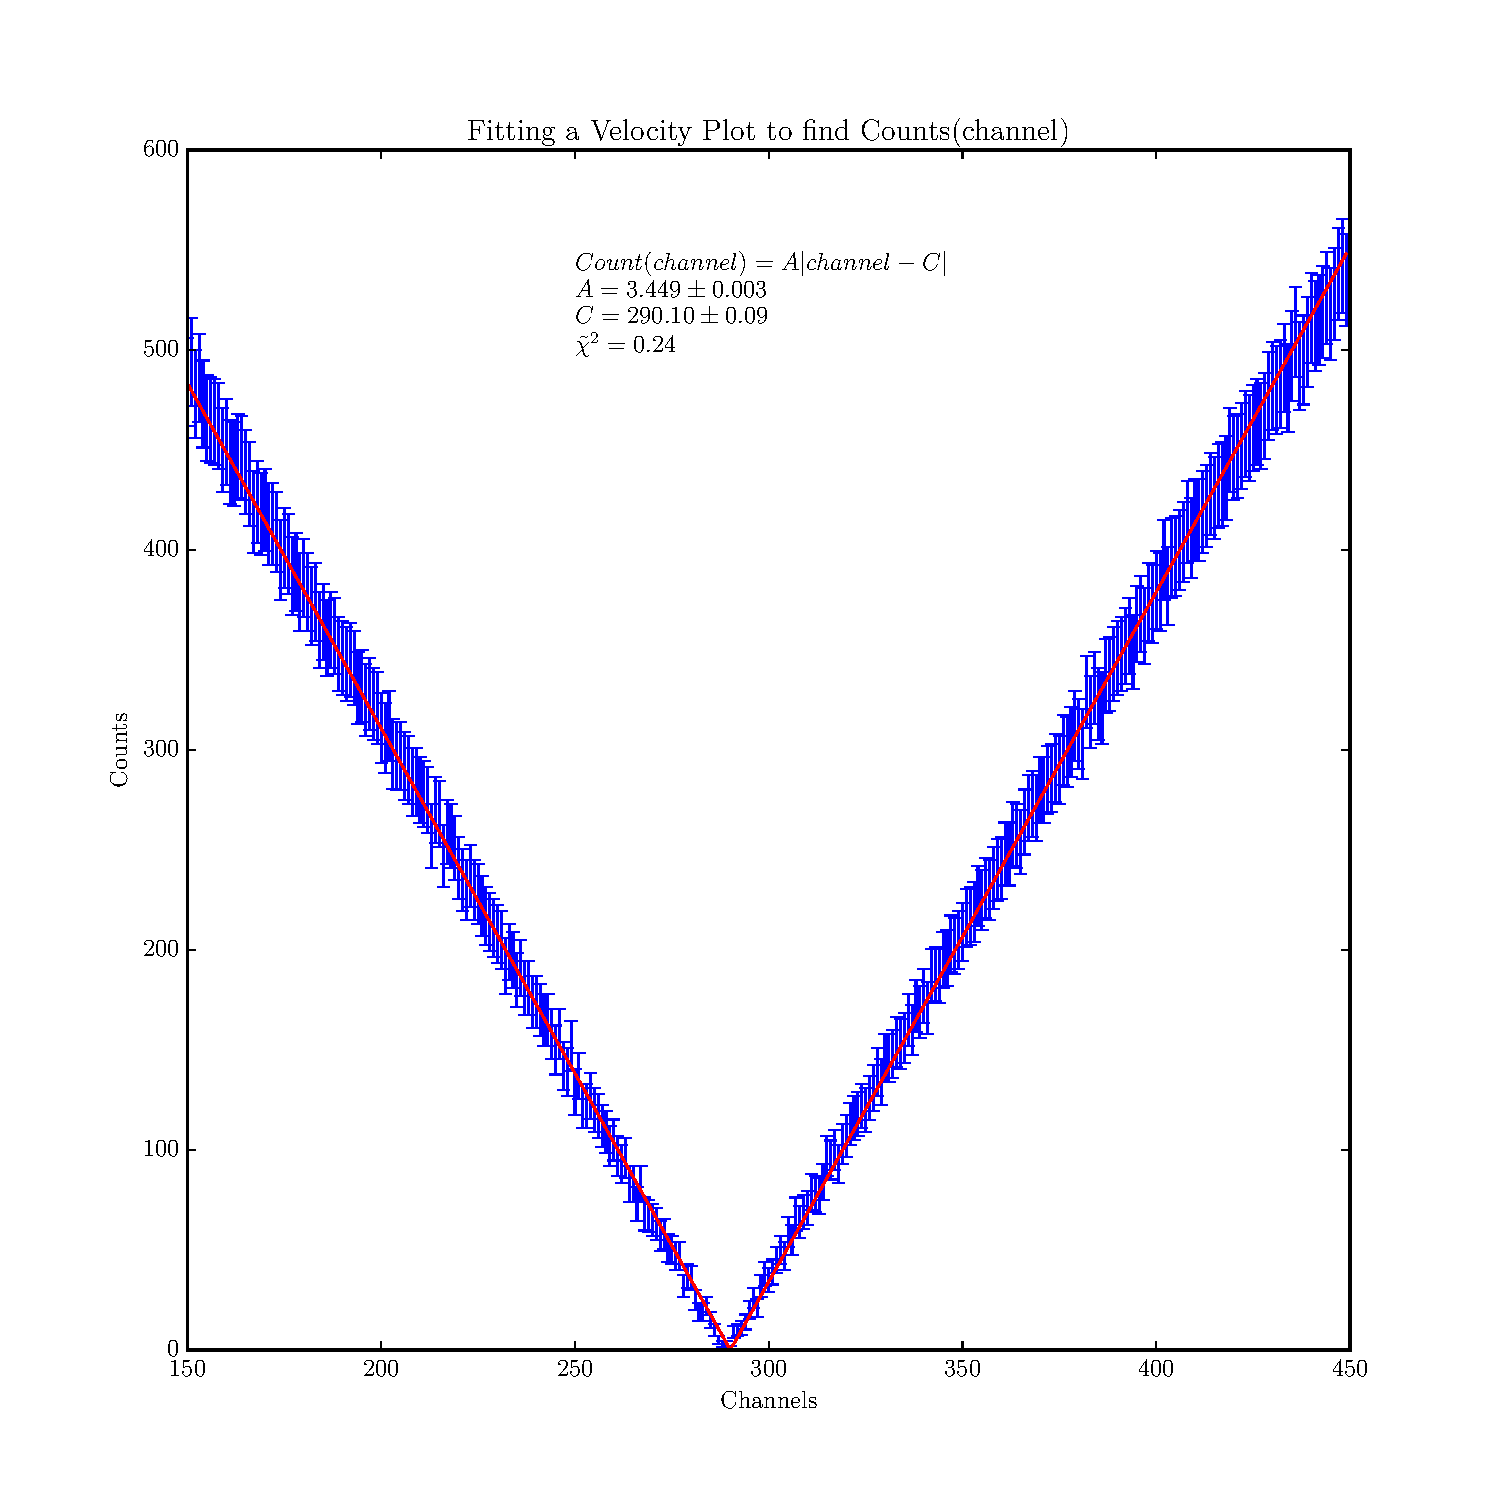
\includegraphics[width=\linewidth]{../plots/velocity.pdf}
        \caption{Fitting to find the counts as a function of channel.  This will allow us to convert channels to velocity, and then from velocity (using the Doppler shift formula) to an energy.  The \redchi value is very low, this is likely due to the large individual point uncertainty (defined as $\sqrt{N}$).  Notice, however, that the fit value uncertainties are tiny - less than 0.01\% in both cases - and this gives us excellent confidence in our fitted values and also allows us to determine that the uncertainty from this calibration is quite negligible.~\label{velocity_plot}}
      \end{figure}

      \begin{figure}[h]
        \centering
        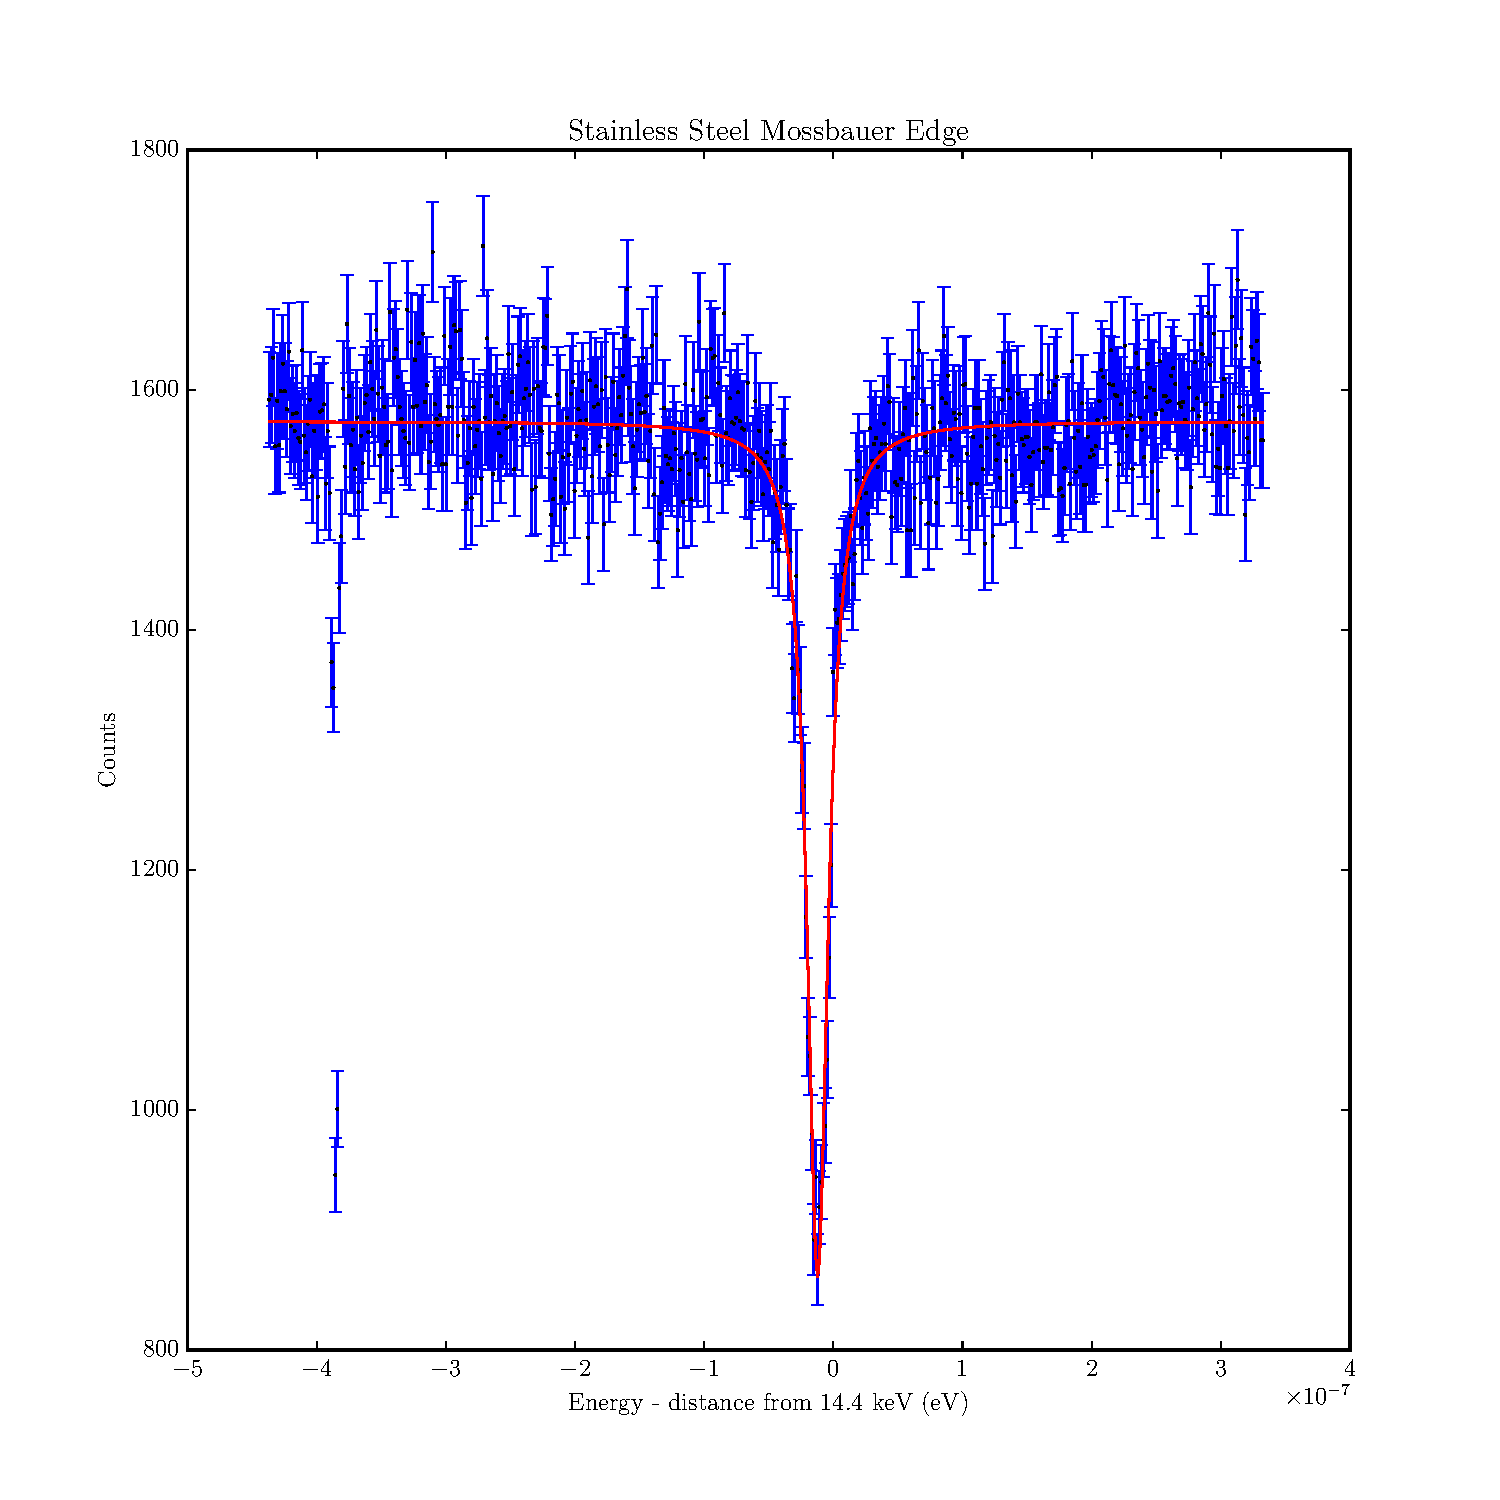
\includegraphics[width=\linewidth]{../plots/ss_fit.pdf}
        \caption{
          Fitting the spectrum for Stainless Steel Grade 302 in order to determine the isomer shift of the Fe-57 contained in the sample.  We fit to the form: \\
            $I(E) = -I_0 \frac{(\Gamma/2)^2}{(E - \delta)^2 + (\Gamma/2)^2}$ \\
          with values held in Table~\ref{tab:ss_fit_stats}.  The \redchi value was a little high, but for a fit with such a large background deviation, we should not be overly worried.  We return for the fit $\tilde{\chi}^2 = 2.09$.  We should note that here and going forward, we use $\delta$ to refer to distance from 0, or in our case, 14.4 keV.  Thus all our values for peak centers are expressed in terms of distance from 14.4 keV.
          ~\label{ss_fit}
        }
      \end{figure}

      \begin{figure}[h]
        \centering
        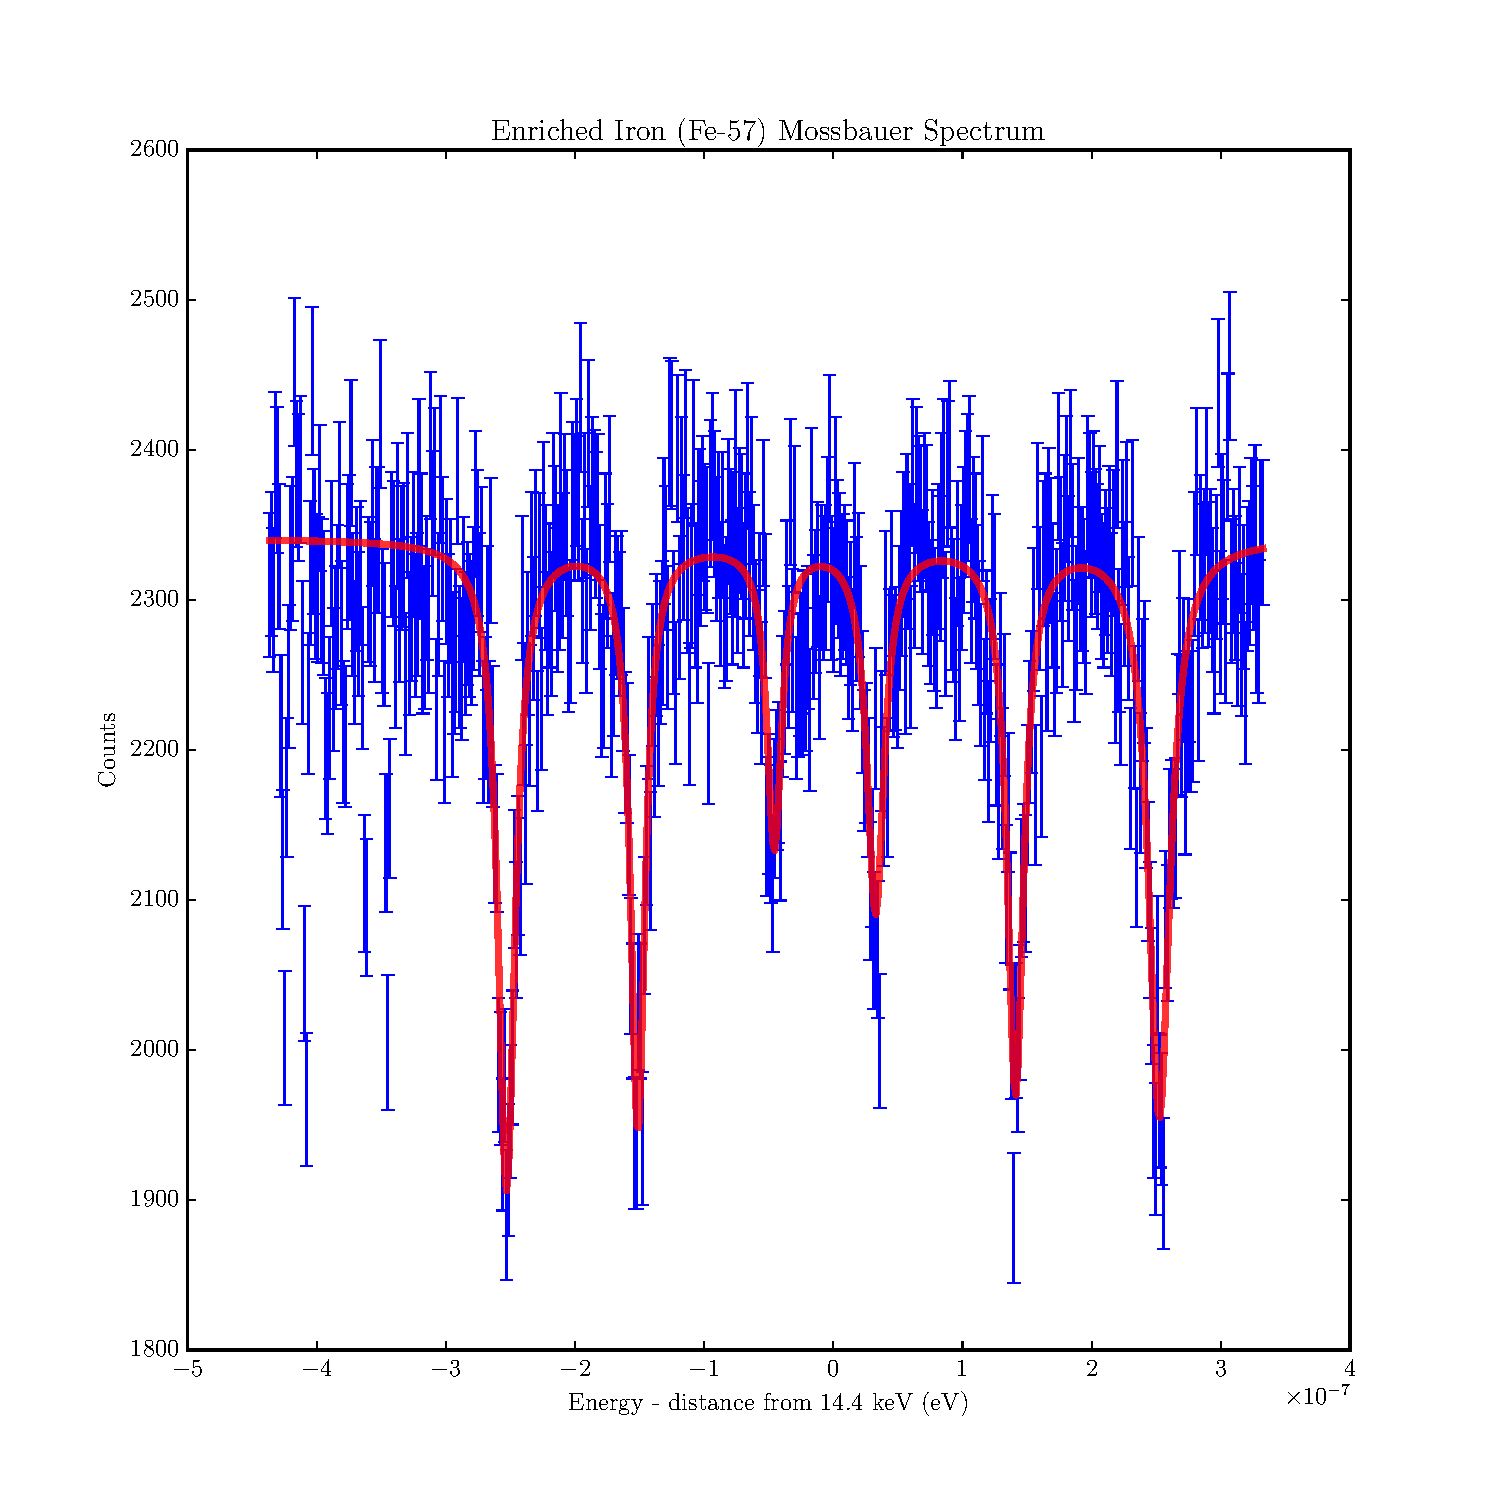
\includegraphics[width=\linewidth]{../plots/fe_fit.pdf}
        \caption{Fitting the spectrum for the Fe-57 sample to determine the Zeeman splitting of the atomic energy levels.  Fit values are held in Table~\ref{tab:fe_57_fit}.  We fit to a function: \\
          $I(E) = C - \sum\limits_{i = 0}^{i = 5}{ \frac{(\Gamma_i/2)^2}{(E-\delta_i)^2 + (\Gamma_i/2)^2} }$ \\
        The \redchi value was an astounding $\tilde{\chi}^2 = 1.71$.  This leads us to believe that the model chosen was indeed correct.~\label{fe_fit}}
      \end{figure}

      \begin{figure}[h]
        \centering
        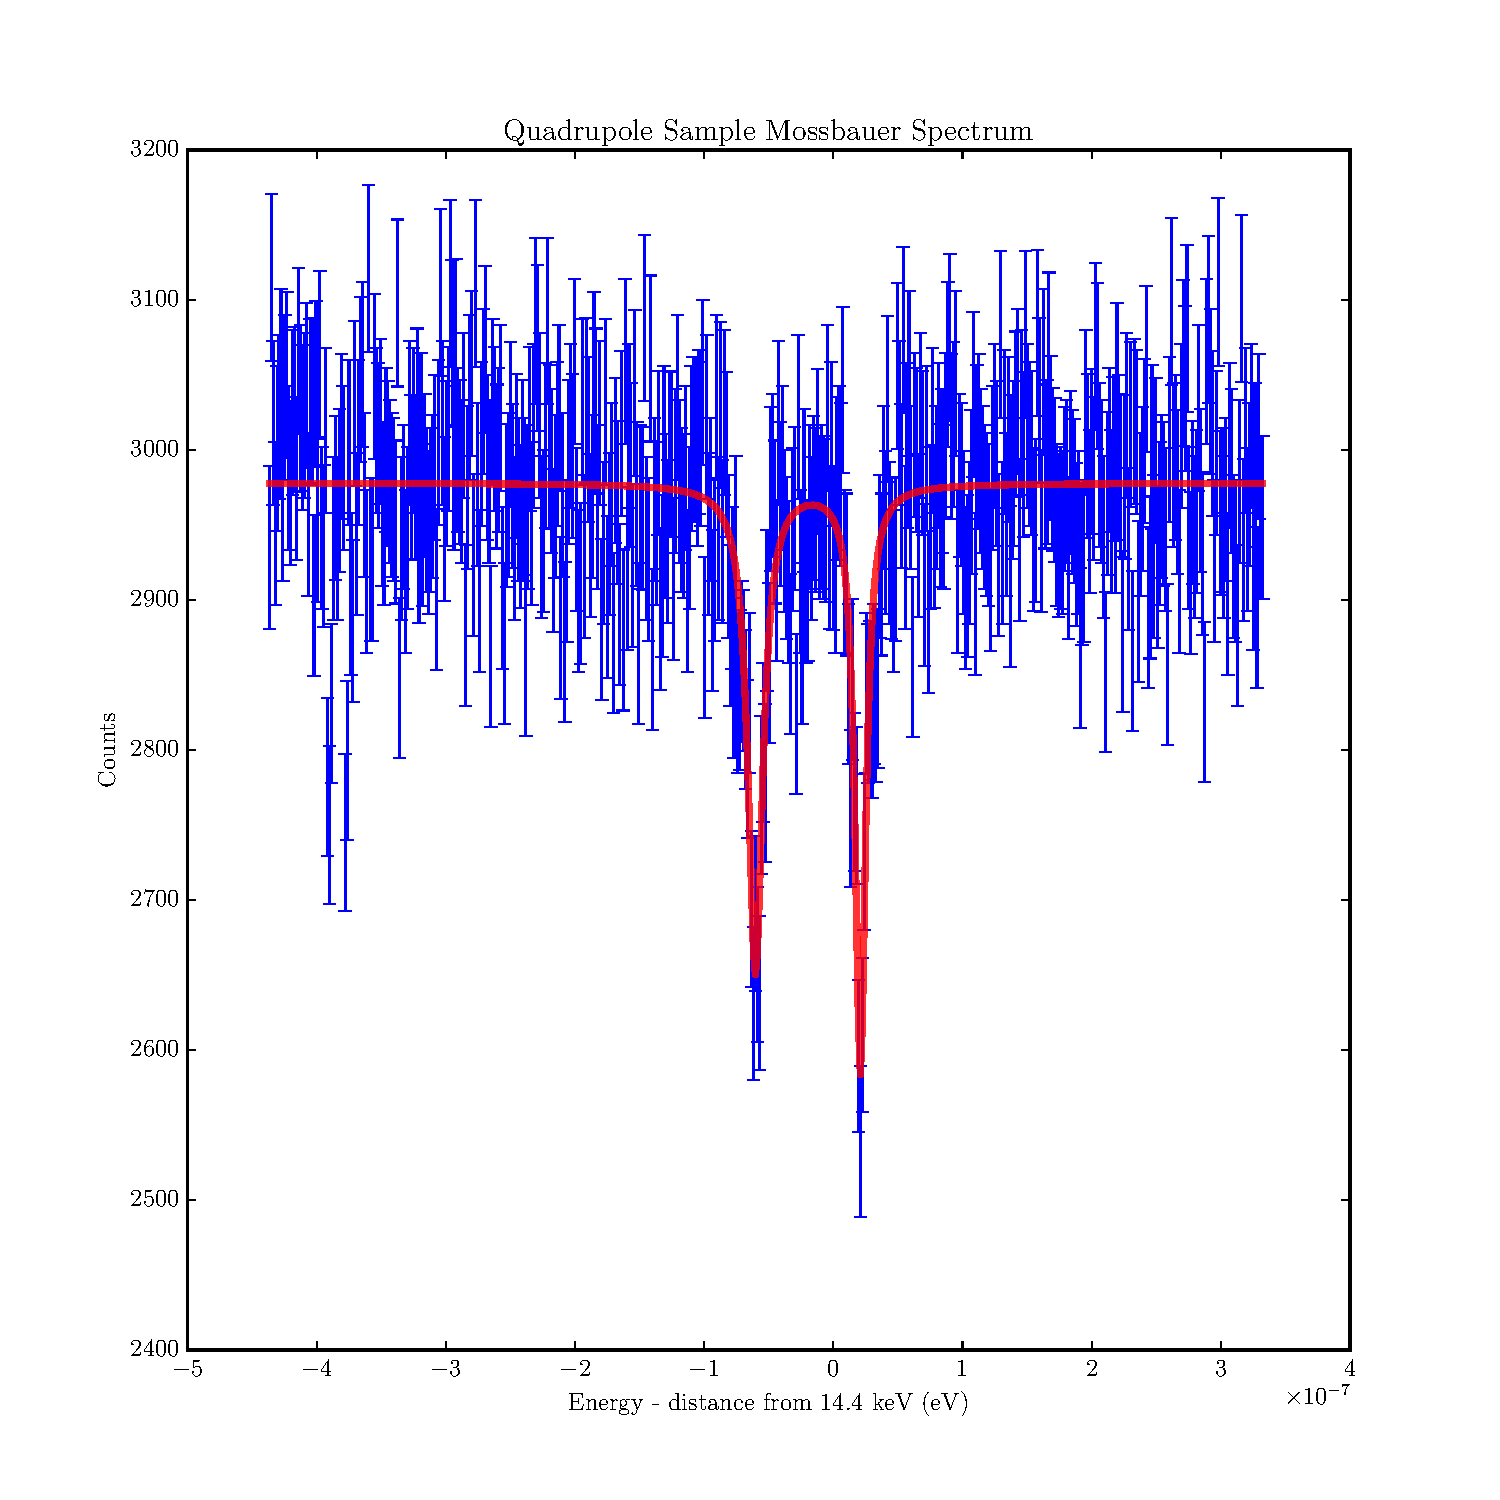
\includegraphics[width=\linewidth]{../plots/quadrupole.pdf}
        \caption{Fitting the spectrum for the Quadrupole sample to determine the quadrupole splitting.  Fit values are held in Table~\ref{tab:quad_fit}.  We fit to a function: \\
          $I(E) = C - \sum\limits_{i = 0}^{i = 1}{ \frac{(\Gamma_i/2)^2}{(E-\delta_i)^2 + (\Gamma_i/2)^2} }$ \\
        The \redchi value was $\tilde{\chi}^2 = 1.07$ which indicates an excellent fit and choice of model.~\label{quadrupole_fit}}
      \end{figure}

    \end{widetext}

    \bibliography{bibliography}
    \bibliographystyle{plain}

\end{document}
